% !Mode:: "TeX:UTF-8"

\begin{frame}
	\frametitle{第七讲、空间曲线}
	\linespread{1.5}
	\begin{enumerate}
	  \item {\bf 内容与要求}{\color{blue}( \S8.4 )}
	  \begin{itemize}
	    \item 熟练掌握空间曲线方程参数化方法
	    \item 熟练掌握投影曲线的方程
	    \item 了解曲面的截痕曲线
% 	    \item 熟练掌握空间平面和直线的方程
% 	    \begin{itemize}
% 	      \item 可分离变量方程
% 	      \item 齐次方程
% 	      \item 一阶线性方程
% 	    \end{itemize}
	  \vspace{1em}
	  \end{itemize}
	  \item {\bf  课后作业:}
	  \begin{itemize}
	    \item {\b 习题8.4:2,4,5,7-11,13}
	  \end{itemize}
	\end{enumerate}
\end{frame}

\begin{frame}[<+->]{复习与回顾}
	\linespread{1.5}
	\begin{enumerate}
	  \item {\bf 空间曲面的参数方程:}2个参数
	  \begin{itemize}
	    \item 球面的极坐标方程
	  \end{itemize}
	  \item {\bf 几类特殊的曲面}
	  \begin{itemize}
	    \item 旋转曲面
	    \item 柱面
	    \item 二次曲面
	    \item 直纹面
	  \end{itemize}
	\end{enumerate}
\end{frame}

\begin{frame}[<+->]
	\linespread{1.2}
	\begin{exampleblock}{{\bf 例1:}判断以下曲面的类型及其特征\hfill}
		\begin{columns}[t]
			\column{.55\textwidth}
				\begin{enumerate}
				  \item $x^2+y^2+z^2+2x-2y=0$
				  \item $x^2-y^2+z^2+2x-2y=0$
				  \item $x^2+y^2+z^2+2x-2y=2$
				  \item $x^2-y^2+z^2+2x-2y=2$
				  \item $x^2-y^2+z^2+2x-2y=-2$
				  \item $x^2+y^2+z^2+2x+2y=2$
				\end{enumerate}
			\column{.45\textwidth}
				\begin{enumerate}
				  \addtocounter{enumi}{6}
				  \item $x^2+y^2-z^2+2xy=0$
				  \item $x^2+y^2-z=0$
				  \item $x^2-y^2-z=0$
				  \item $x^2-z=0$
				  \item $x^2-y+z=0$
				\end{enumerate}
		\end{columns}
	\end{exampleblock}
\end{frame}

% \begin{frame}{双曲抛物面(马鞍面)}
% 	\linespread{1.2}\pause 
% 	$$\alert{z=\df{x^2}{a^2}-\df{y^2}{b^2}}$$\pause 
% 	\begin{center}
% 		\resizebox{!}{4cm}{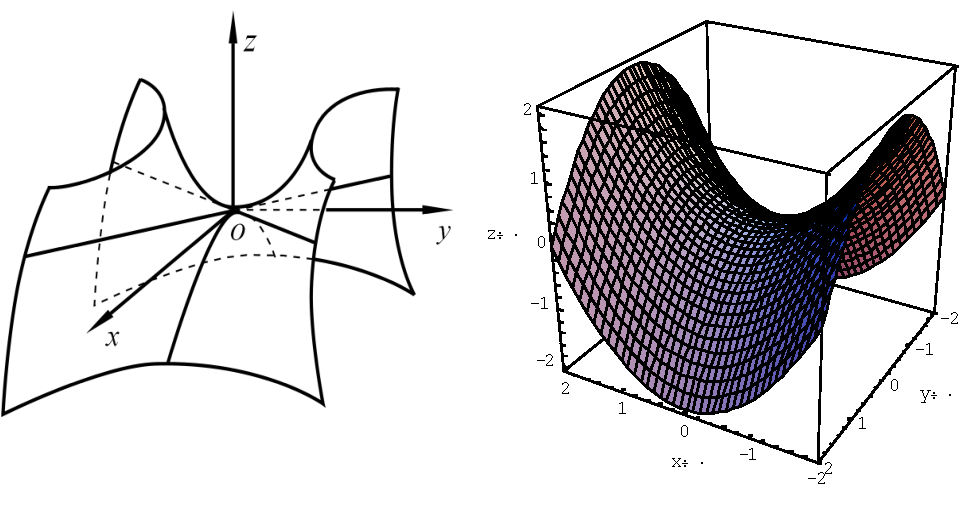
\includegraphics{./images/ch8/quaArch.pdf}}
%  	\end{center}\pause 
%  	\vspace{-1em}
%  	$$\alert{x=au\sec\theta,\;y=bu\tan\theta,\;z=u^2}$$
%  	$$\alert{(0\leq\theta\leq 2\pi,u\geq 0)}$$
% \end{frame}
% 
% \begin{frame}
% 	\linespread{1.2}
% 	\begin{exampleblock}{{\bf 例2}\hfill P52-例12}
% 		证明:$z=xy$对应的曲面为双曲抛物面
% 	\end{exampleblock}\pause 
% 	\begin{center}
% 		\resizebox{!}{4cm}{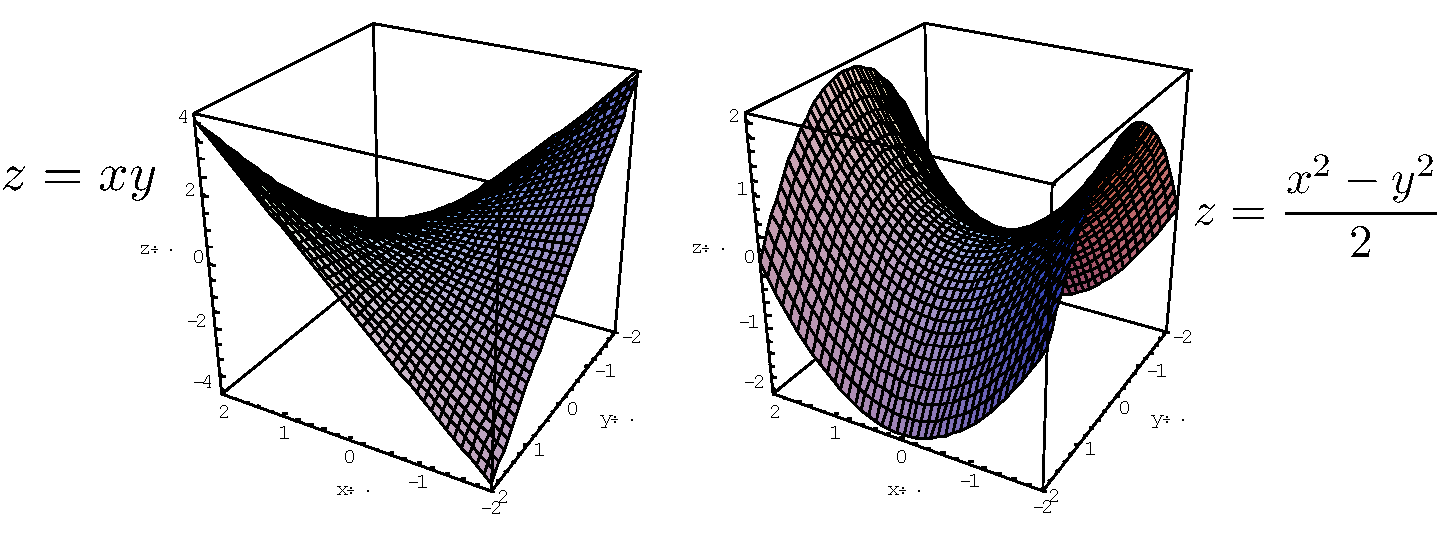
\includegraphics{./images/ch8/diffArch.pdf}}
%  	\end{center}\pause 
%  	{\bb (二维)坐标旋转公式:}{\b (逆时针旋转$\theta$)}
%  	$$\alert{\left\{\begin{array}{l}
%  		X=x\cos\theta+y\sin\theta\\
%  		Y=-x\sin\theta+y\cos\theta
%  	\end{array}\right.}$$
% \end{frame}
% 
% \begin{frame}{直纹面}
% 	\linespread{1.2}
% 	\ba{空间直线按照一定的规律运动会产生什么样的曲面?}\pause 
% 	\begin{center}
% 		\resizebox{!}{5cm}{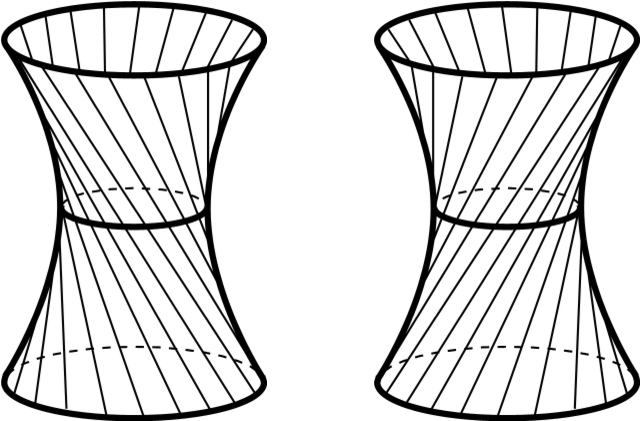
\includegraphics{./images/ch8/rtLHypo.pdf}}
% 		
% 		{\b 单叶双曲面}(习题8.3-10)
%  	\end{center}
% \end{frame}

\section{空间曲线}

\begin{frame}{空间曲线的参数方程}
	\linespread{1.2}\pause 
	\ba{任意曲线都可以视为动点的运动轨迹}\pause 
% 	
% 	{\bf 参数:}时间$t$
% 	
% 	{\bf 参数方程:}
	$$\alert{x=x(t),\;y=y(t),\;z=z(t)}$$\pause 
	\begin{exampleblock}{{\bf 例3:}以下方程表示何种曲线\hfill P57-例1}\pause 
		\begin{enumerate}
		  \item $x=\cos t,\;y=\sin t,\;z=t\;(t\in\mathbb{R})$\pause 
		  \item $x=t\cos t,\;y=t\sin t,\;z=t\;(t\in\mathbb{R})$ 
		\end{enumerate}
	\end{exampleblock}
\end{frame}

\begin{frame}{空间曲线的一般式方程}
	\linespread{1.2}\pause 
	\ba{空间曲线可视为两个(或更多)曲面的交线}\pause 
	$$\alert{\left\{\begin{array}{l}
		F(x,y,z)=0,\\ G(x,y,z)=0
	\end{array}\right.}$$\pause 
	\begin{exampleblock}{{\bf 例4:}以下方程对应何种曲线\hfill P59-例3}
		$$\left\{\begin{array}{l}
			z=\sqrt{R^2-x^2-y^2},\\ x^2+y^2-Rx=0
		\end{array}\right.\pause \quad{\b \mbox{(Viviani曲线)}}$$
	\end{exampleblock}
\end{frame}

\section{空间曲线的投影}

\begin{frame}{空间曲线的投影}
	\linespread{1.2}\pause 
	\begin{exampleblock}{{\bf 例5}\hfill P60-例5}
		求空间曲线$C:\left\{\begin{array}{l}
			x^2+y^2+z^2=1\\ x^2+(y-1)^2+(z-1)^2=1
		\end{array}\right.$
		在$xOy$平面上的投影曲线方程。
	\end{exampleblock}\pause 
	\begin{columns}
		\column{.55\textwidth}
			\begin{center}
				\resizebox{!}{3.5cm}{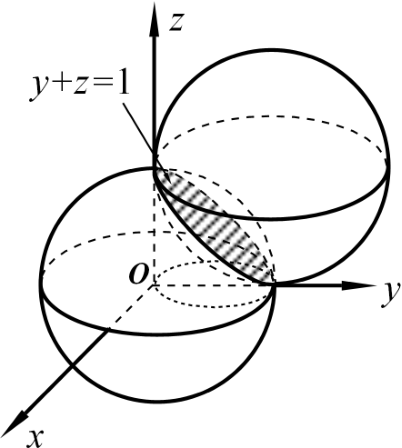
\includegraphics{./images/ch8/shaBall.pdf}}
			\end{center}\pause 
		\column{.45\textwidth}
			\ba{曲线在$xOy$上的投影=变量$x,y$满足的柱面方程与$xOy$平面的交线}
	\end{columns}
\end{frame}

\begin{frame}{空间曲线的投影}
	\linespread{1.2}\pause 
	空间曲线:
	$$C:\left\{\begin{array}{l}
		F(x,y,z)=0\\ G(x,y,z)=0
	\end{array}\right.$$\pause 
	消去$z$,所得方程
	$$H(x,y)=0$$\pause 
	\vspace{-1em}
	\begin{itemize}
	  \item 曲线$C$关于$xOy$平面的\ba{投影柱面}\pause 
	  \item $xOy$平面内的一条曲线——\ba{$C$的投影曲线}
	\end{itemize}
\end{frame}

\begin{frame}{参数方程与投影曲线}
	\linespread{1.2}\pause 
	{\bf 曲线$C$:}
	$$x=x(t),\;y=y(t),\;z=z(t)\;(t\in[t_0,t_1])$$\pause 
	{\bf 曲线$C$在$xOy$平面内的投影曲线:}
	$$x=x(t),\;y=y(t),\;\alert{z=0}\;(t\in[t_0,t_1])$$\pause 
	{\bf 思考:}{\b 如果直接在曲线的一般式方程中令$z=0$,所得是否即为其在$xOy$平面内的投影曲线?}\pause
	($\alert{\times}$)
\end{frame}

\begin{frame}
	\linespread{1.2}
	\begin{exampleblock}{{\bf 例6}\hfill P59-例4}
		圆柱螺旋线在三个坐标面上的投影分别是什么曲线?
	\end{exampleblock}
	\pause
	\begin{columns}
		\column{.5\textwidth}
			\begin{center}
				\resizebox{!}{5cm}{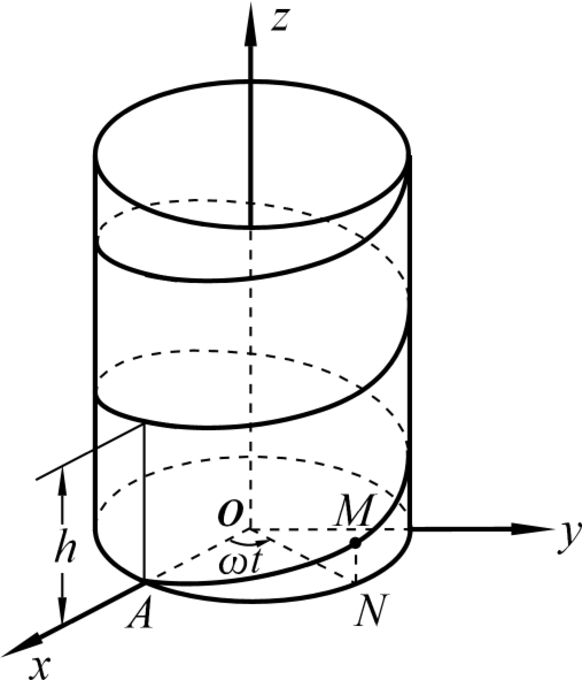
\includegraphics{./images/ch8/cylinderCurve.pdf}}
			\end{center}\pause 
		\column{.45\textwidth}
			$$\alert{\left\{\begin{array}{l}
					x=R\sin t\\ y=R\cos t\\ z=at
				\end{array}\right.\;(t\in\mathbb{R})}$$
	\end{columns}
\end{frame}

\begin{frame}
	\linespread{1.2}
	\begin{exampleblock}{{\bf 例7}\hfill P61-例6}
		求Viviani曲线在各坐标面上的投影曲线,并由此写出Viviani曲线的参数方程。
	\end{exampleblock}\pause 
	\begin{columns}
		\column{.5\textwidth}
			\begin{center}
				\resizebox{!}{4.5cm}{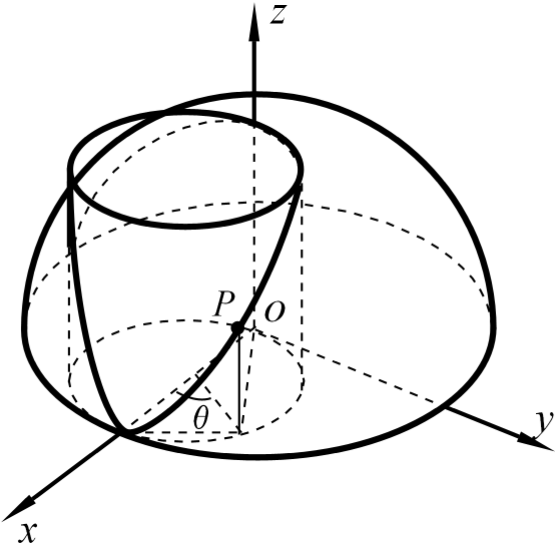
\includegraphics{./images/ch8/viviani.pdf}}
			\end{center}\pause 
		\column{.45\textwidth}
			$$\alert{\left\{\begin{array}{l}
				z=\sqrt{R^2-x^2-y^2}\\
				x^2+y^2-Rx=0
			\end{array}\right.}$$
	\end{columns}
\end{frame}

\begin{frame}
	\linespread{1.2}
	\begin{center}
		\resizebox{!}{6.5cm}{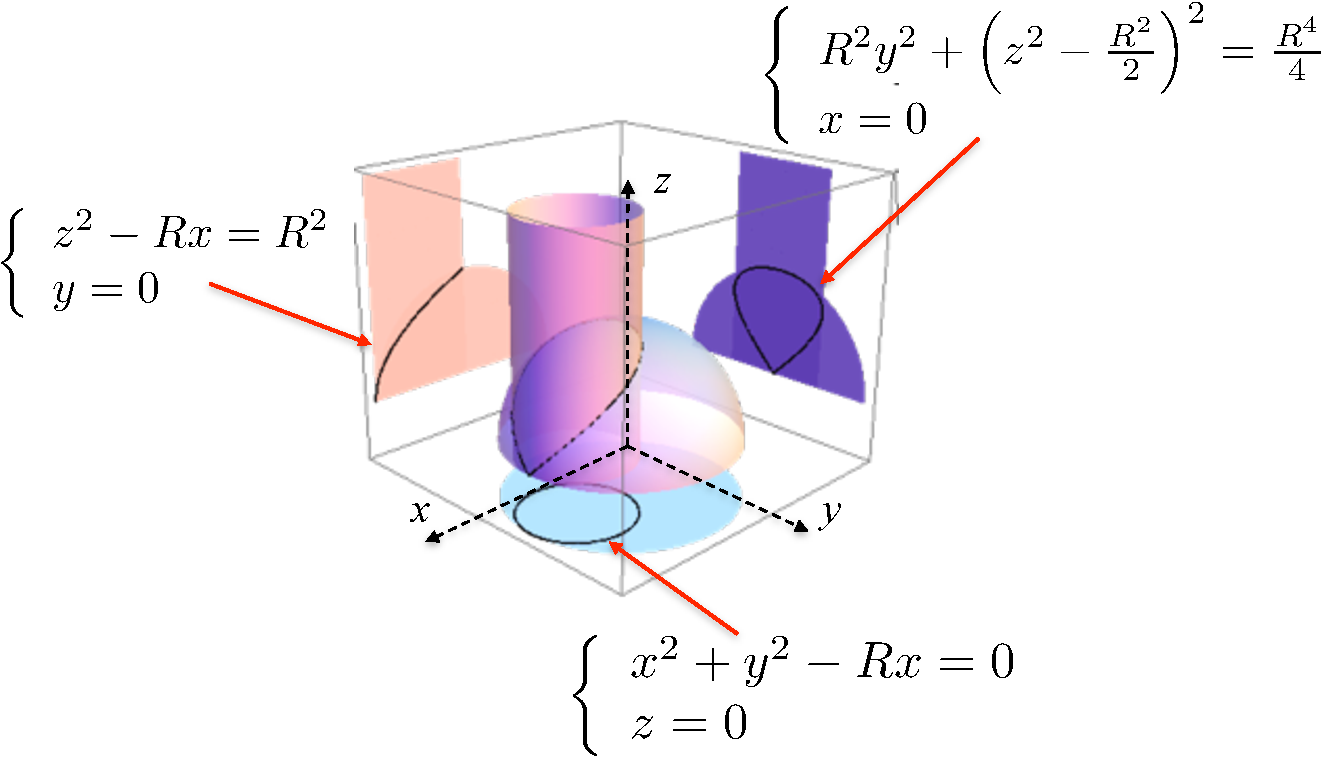
\includegraphics{./images/ch8/vivianiPara.pdf}}
	\end{center}\pause 
	\vspace{-1ex}
	$$\alert{x=\df R2(1+\cos\theta),\;y=\df
	R2\sin\theta,\;z=R\sin\df{\theta}{2},\;\theta\in[0,2\pi]}$$
\end{frame}

\section{曲面的截痕曲线}

\begin{frame}{曲面的截痕曲线}
	\linespread{1.2}\pause 
	{\bb 截痕曲线:}特定平面与曲面的交线\pause 
	\begin{exampleblock}{{\bf 例8}\hfill}
		试用考查以下曲面的截痕曲线:
		\begin{enumerate}
		  \item 单叶双曲面
		  \item 双叶双曲面
		  \item 双曲抛物面
		\end{enumerate}
	\end{exampleblock}
\end{frame}

\begin{frame}[<+->]{小结}
	\linespread{1.5}
	\begin{enumerate}
	  \item {\bf 空间曲线的方程}
	  \begin{itemize}
	    \item 参数方程
	    \item 一般式方程
	  \end{itemize}
	  \item {\bf 空间曲线的投影}
	  \begin{itemize}
	    \item 由投影曲线方程求曲线的参数方程
	  \end{itemize}
	\end{enumerate}
\end{frame}

\begin{frame}{补充例题}
	\linespread{1.2}
	\begin{exampleblock}{{\bf 例9}\hfill}
		求与直线$y=0,z=a$和$x=0,z=-a$均相切的球面中心的轨迹,并判断其形状。
	\end{exampleblock}
\end{frame}

\begin{frame}
	\linespread{1.2}
	\begin{exampleblock}{{\bf 例10}\hfill}
		求直线
		$$l:\df{x}{a}=\df{y-b}0=z$$绕$z$轴旋转一周所得曲面方程,并指出该曲面
		的类型。
	\end{exampleblock}
\end{frame}

\begin{frame}
	\linespread{1.2}
	\begin{exampleblock}{{\bf 例11}\hfill}
		求曲线$\left\{\begin{array}{l}
			x^2-y^2=2z+1\\
			x+y=z
		\end{array}\right.$
		的参数方程。
	\end{exampleblock}
\end{frame}

\begin{frame}
	\linespread{1.2}
	\begin{exampleblock}{{\bf 例12}\hfill}
		已知两点$A(1,0,0)$和$B(0,1,1)$,求直线$AB$绕$z$轴旋转一周所得曲面的面积。
	\end{exampleblock}
\end{frame}

\begin{frame}
	\linespread{1.2}
	\begin{exampleblock}{{\bf 例13}\hfill}
		求由不等式组
		$$x\geq 0,\;y\geq 0,\;z\geq 0,\;x+z\leq 1,\; y^2+z^2\leq 1$$
		所确定的立体体积。
	\end{exampleblock}
\end{frame}

\begin{frame}
	\linespread{1.5}
	\begin{exampleblock}{{\bf 例14}\hfill}
		由椭球面$\df{x^2}{a^2}+\df{y^2}{b^2}+\df{z^2}{c^2}=1$的中心引三条相互垂直的射线,
		分别交椭球面于三点$P_i(i=1,2,3)$,记$|\bm{OP}_i|=r_i(i=1,2,3)$,证明:
		$$\df{1}{r_1^2}+\df{1}{r_2^2}+\df{1}{r_3^2}
		=\df{1}{a^2}+\df{1}{b^2}+\df{1}{c^2}$$
	\end{exampleblock}
\end{frame}

% \begin{frame}{title}
% 	\linespread{1.2}
% 	\begin{block}{{\bf title}\hfill}
% 		123
% 	\end{block}
% \end{frame}

% \begin{frame}{title}
% 	\linespread{1.2}
% 	\begin{block}{{\bf title}\hfill}
% 		123
% 	\end{block}
% \end{frame}